\chapter{Forecasting Models}\label{ch:forecast}

The target is $Y_t = S_{t+h}$ for $h$ = 1, 6 and 24 intervals (5 minutes, 30 minutes and 2 hours). Every forecast may only use
what is known at the end of interval $t$.

\section{Features}\label{sec:features}
Features come in eight groups:
\begin{itemize}
\item \textbf{own price}: the price now, its lags, the price at the target time yesterday, and the trailing maximum, mean and
standard deviation over 30 minutes, 2 hours and a day
\item \textbf{excitation}: decaying counts of recent onsets, $E_t = \sum_{s \le t} 2^{-(t-s)/HL}\,\text{onset}_s$ for half lives
of 30 minutes, 3 hours and a day (the excitation term of the Hawkes intensity), the spikes in the last day, and the time since the last spike
\item \textbf{supply}: demand and its ramp, the generation margin, wind and solar availability, net interchange, dispatch error and batteries
\item \textbf{fcas}: the raise regulation and raise 6 second prices, and the cumulative price that triggers administered pricing
\item \textbf{neighbours}: the other regions' prices, how many are spiking, and the highest price in the NEM
\item \textbf{network}: every column of the system table
\item \textbf{constraints}: the 20 individual constraints with the highest mutual information with the target, picked inside
each training set among those binding at least 50 times
\item \textbf{calendar}: time of day and weekend flag of the target interval
\end{itemize}
Prices go in as $\operatorname{asinh}(p/50)$, which is roughly linear near zero, logarithmic for large $|p|$, and fine with negative
prices. The excitation features satisfy $E_t = dE_{t-1} + \text{onset}_t$ with $d = 2^{-1/HL}$, so they are computed in $O(N)$.
The fitted Hawkes half lives, $\ln 2/\beta$, are about 30 minutes in NSW1, QLD1 and VIC1 and about an hour in SA1 and TAS1,
which the 30 minute and 3 hour features bracket. To check nothing looks into the future, every input after some time $t$ is
replaced by noise, and we verify that no feature at or before $t$ changes.

\section{Models}
We compare three models.
\begin{itemize}
\item \textbf{Persistence}: $p = g(\text{price now})$ with $g$ non-decreasing, fitted by isotonic regression. It assumes only that
a higher price now never makes a spike less likely. A seasonal climatology and a two state Markov chain were also tried, and
Persistence had the higher AP in every region and at every horizon.
\item \textbf{Logistic}: L2 penalised logistic regression, $C = 0.1$, on standardised features.
\item \textbf{Boosting trees} (GBM): described below.
\end{itemize}

\subsection{Boosting Trees}
Gradient boosting \cite{friedman2001} builds the log odds of a spike as a sum of small regression trees, each fitted to the
errors of the ones before. We use LightGBM \cite{ke2017} with 200 trees of 7 leaves and learning rate 0.02. Two choices matter a
lot, because for SA1, TAS1 and VIC1 the training months saw few extreme prices and the winter test months saw many:
\begin{itemize}
\item boosting \emph{starts from} the Persistence log odds, so the trees only learn corrections to ``a high price now means a
spike soon'': $\operatorname{logit} p = \operatorname{logit} g(\text{price now}) + \sum_k f_k(x)$
\item monotone constraints force the prediction to go up with price, excitation and neighbour spike features, and down with the
supply margin and the time since the last spike. Otherwise the trees can learn ``a price above anything seen in training means no spike''.
\end{itemize}

\section{Evaluation}
We test walk-forward, one month at a time. The test months are January to September 2026, and for each one the training set is every forecast whose target is before the month starts, so September to December 2025 is only ever training
data. Training sets grow from about 31,000 intervals to about 101,000, and stacking the test months gives about 73,400 out of sample forecasts per region and horizon. Forecasts whose origin or target falls in the 10 March gap are dropped.

Spikes are rare, so accuracy is useless: always predicting ``no spike'' is 98 to 99.97\% accurate. The headline score is
\textbf{average precision} (AP), the area under the precision--recall curve \cite{saito2015}, for which a no skill forecast scores
the base rate. We also report AP over origins not currently spiking (\textbf{AP onset}, predicting that a spike starts), ROC AUC,
and the Brier skill score against always forecasting the base rate. For an alert rule, an alert is raised when
$p$ is above the threshold that maximised F1 on all earlier test months, and we report its precision, recall, F1, and the share
of the cost above \$300/MWh that falls in alerted intervals.

\section{Results}
At 30 minutes the GBM has the best AP in NSW1 (0.52 against 0.37 for Persistence), and only just in SA1 and VIC1, by less than
0.01 (Table \ref{tab:scores}). In QLD1 and TAS1 Persistence is better. So most of what can be predicted half an hour ahead is ``the
price is already high'', and the extra features clearly pay off only in NSW1. Predicting the \emph{start} of a spike is much
harder: AP onset is at most 0.21. Logistic regression falls well behind both.

\begin{table}[!htbp]\centering\small
\caption{Out of sample scores 30 minutes ahead, January to September 2026. Best AP per region in bold.}\label{tab:scores}
\resizebox{\textwidth}{!}{\begin{tabular}{llrrrrrrrrr}
\toprule
 & & base\_rate & AP & AP\_onset & ROC & BSS & precision & recall & F1 & excess\_capture \\
region & model & & & & & & & & & \\
\midrule
\multirow[t]{3}{*}{NSW1} & Persistence & 0.002 & 0.369 & 0.138 & 0.982 & 0.256 & 0.263 & 0.448 & 0.331 & 0.359 \\
 & Logistic & 0.002 & 0.267 & 0.116 & 0.949 & 0.046 & 0.283 & 0.344 & 0.310 & 0.355 \\
 & GBM & 0.002 & 0.452 & 0.193 & 0.992 & 0.298 & 0.444 & 0.352 & 0.393 & 0.331 \\
\cline{1-11}
\multirow[t]{3}{*}{QLD1} & Persistence & 0.000 & 0.056 & 0.030 & 0.943 & 0.025 & 0.015 & 0.042 & 0.022 & 0.001 \\
 & Logistic & 0.000 & 0.058 & 0.012 & 0.921 & -0.098 & 0.154 & 0.083 & 0.108 & 0.008 \\
 & GBM & 0.000 & 0.057 & 0.036 & 0.976 & 0.024 & 0.000 & 0.000 & 0.000 & 0.000 \\
\cline{1-11}
\multirow[t]{3}{*}{SA1} & Persistence & 0.019 & 0.736 & 0.167 & 0.976 & 0.493 & 0.602 & 0.653 & 0.626 & 0.313 \\
 & Logistic & 0.019 & 0.317 & 0.035 & 0.779 & 0.203 & 0.213 & 0.387 & 0.275 & 0.204 \\
 & GBM & 0.019 & 0.717 & 0.176 & 0.981 & 0.433 & 0.508 & 0.675 & 0.580 & 0.313 \\
\cline{1-11}
\multirow[t]{3}{*}{TAS1} & Persistence & 0.001 & 0.358 & 0.035 & 0.882 & 0.219 & 0.534 & 0.330 & 0.408 & 0.432 \\
 & Logistic & 0.001 & 0.027 & 0.003 & 0.827 & -0.361 & 0.038 & 0.096 & 0.054 & 0.304 \\
 & GBM & 0.001 & 0.225 & 0.029 & 0.913 & 0.086 & 0.206 & 0.074 & 0.109 & 0.032 \\
\cline{1-11}
\multirow[t]{3}{*}{VIC1} & Persistence & 0.003 & 0.580 & 0.132 & 0.993 & 0.334 & 0.453 & 0.457 & 0.455 & 0.625 \\
 & Logistic & 0.003 & 0.146 & 0.019 & 0.865 & 0.057 & 0.069 & 0.327 & 0.113 & 0.613 \\
 & GBM & 0.003 & 0.615 & 0.128 & 0.994 & 0.320 & 0.369 & 0.482 & 0.418 & 0.636 \\
\cline{1-11}
\bottomrule
\end{tabular}}
\end{table}

\textbf{Is the GBM really better?} A test month only holds a few dozen spike episodes, so we use a day block bootstrap
\cite{kunsch1989}: resample whole days 500 times and recompute AP.

\begin{table}[!htbp]\centering\small
\caption{Day block bootstrap of AP, 30 minutes ahead (500 resamples).}\label{tab:bootstrap}
\resizebox{\textwidth}{!}{\begin{tabular}{llrrrrrr}
\toprule
 & & AP\_lo & AP\_med & AP\_hi & GBM\_minus\_lo & GBM\_minus\_hi & P(GBM better) \\
region & model & & & & & & \\
\midrule
\multirow[t]{3}{*}{NSW1} & Persistence & 0.123 & 0.365 & 0.531 & -0.033 & 0.164 & 0.926 \\
 & Logistic & 0.028 & 0.270 & 0.534 & 0.019 & 0.353 & 0.988 \\
 & GBM & 0.091 & 0.452 & 0.615 & NaN & NaN & NaN \\
\cline{1-8}
\multirow[t]{3}{*}{QLD1} & Persistence & 0.004 & 0.054 & 0.200 & -0.043 & 0.036 & 0.470 \\
 & Logistic & 0.003 & 0.056 & 0.155 & -0.028 & 0.044 & 0.568 \\
 & GBM & 0.006 & 0.056 & 0.176 & NaN & NaN & NaN \\
\cline{1-8}
\multirow[t]{3}{*}{SA1} & Persistence & 0.503 & 0.729 & 0.845 & -0.067 & 0.020 & 0.156 \\
 & Logistic & 0.067 & 0.313 & 0.549 & 0.242 & 0.503 & 1.000 \\
 & GBM & 0.469 & 0.712 & 0.834 & NaN & NaN & NaN \\
\cline{1-8}
\multirow[t]{3}{*}{TAS1} & Persistence & 0.006 & 0.357 & 0.702 & -0.217 & 0.006 & 0.144 \\
 & Logistic & 0.001 & 0.026 & 0.149 & 0.004 & 0.489 & 1.000 \\
 & GBM & 0.006 & 0.217 & 0.555 & NaN & NaN & NaN \\
\cline{1-8}
\multirow[t]{3}{*}{VIC1} & Persistence & 0.218 & 0.569 & 0.795 & -0.075 & 0.235 & 0.602 \\
 & Logistic & 0.008 & 0.138 & 0.449 & 0.145 & 0.647 & 1.000 \\
 & GBM & 0.171 & 0.598 & 0.838 & NaN & NaN & NaN \\
\cline{1-8}
\bottomrule
\end{tabular}}
\end{table}

\textbf{Horizons.} Skill drops quickly with the horizon (Figure \ref{fig:horizon}). Five minutes ahead spikes are very
predictable, with AP up to 0.86 against base rates below 2\%. By 2 hours AP is below 0.2 everywhere except SA1 (0.54), where
episodes last long enough that the price now still says something. The GBM's lead over Persistence grows with the horizon: at
2 hours it has the best AP in every region, most clearly in NSW1 (0.20 against 0.07), as the current price says less and the
other features have more to add.

\begin{figure}[!htbp]\centering
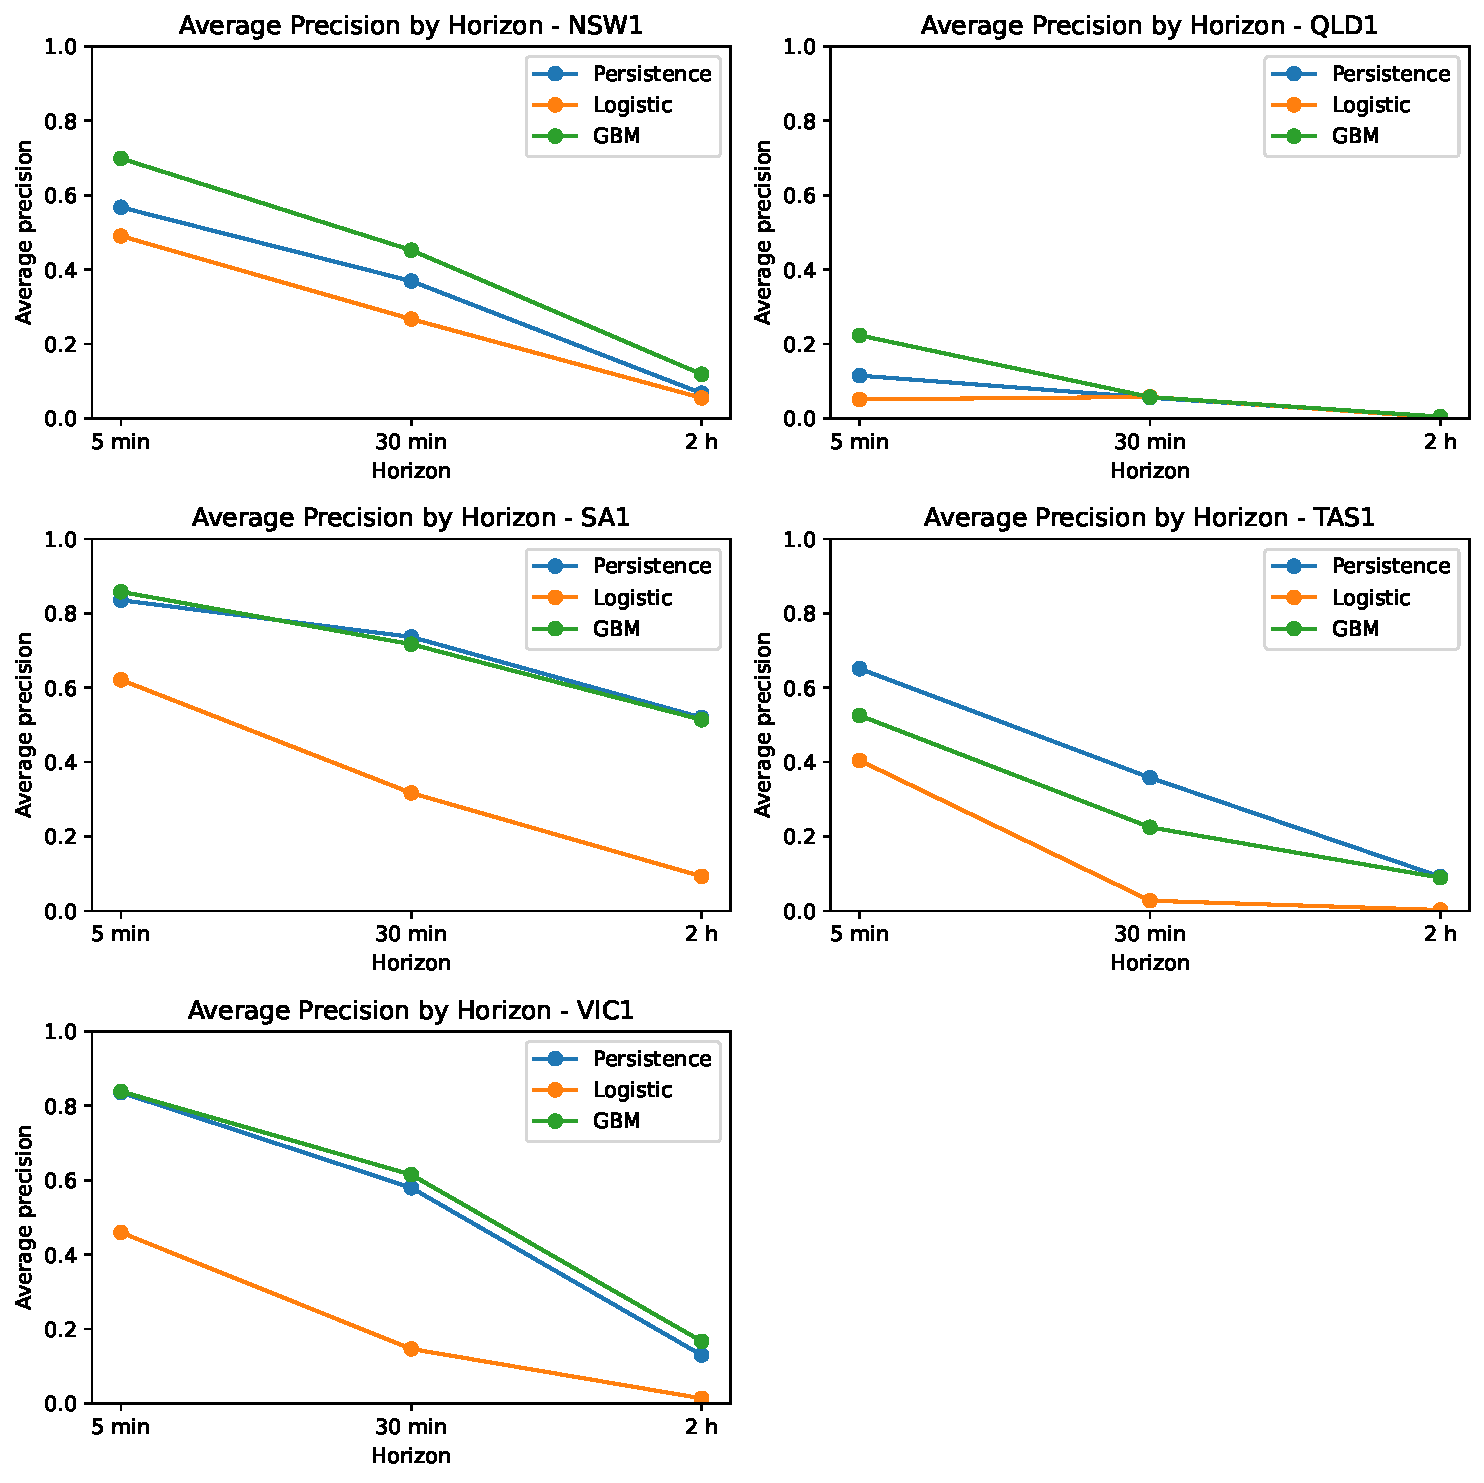
\includegraphics[width=0.8\textwidth]{ap_vs_horizon.pdf}
\caption{Average precision against horizon.}\label{fig:horizon}
\end{figure}

\begin{figure}[!htbp]\centering
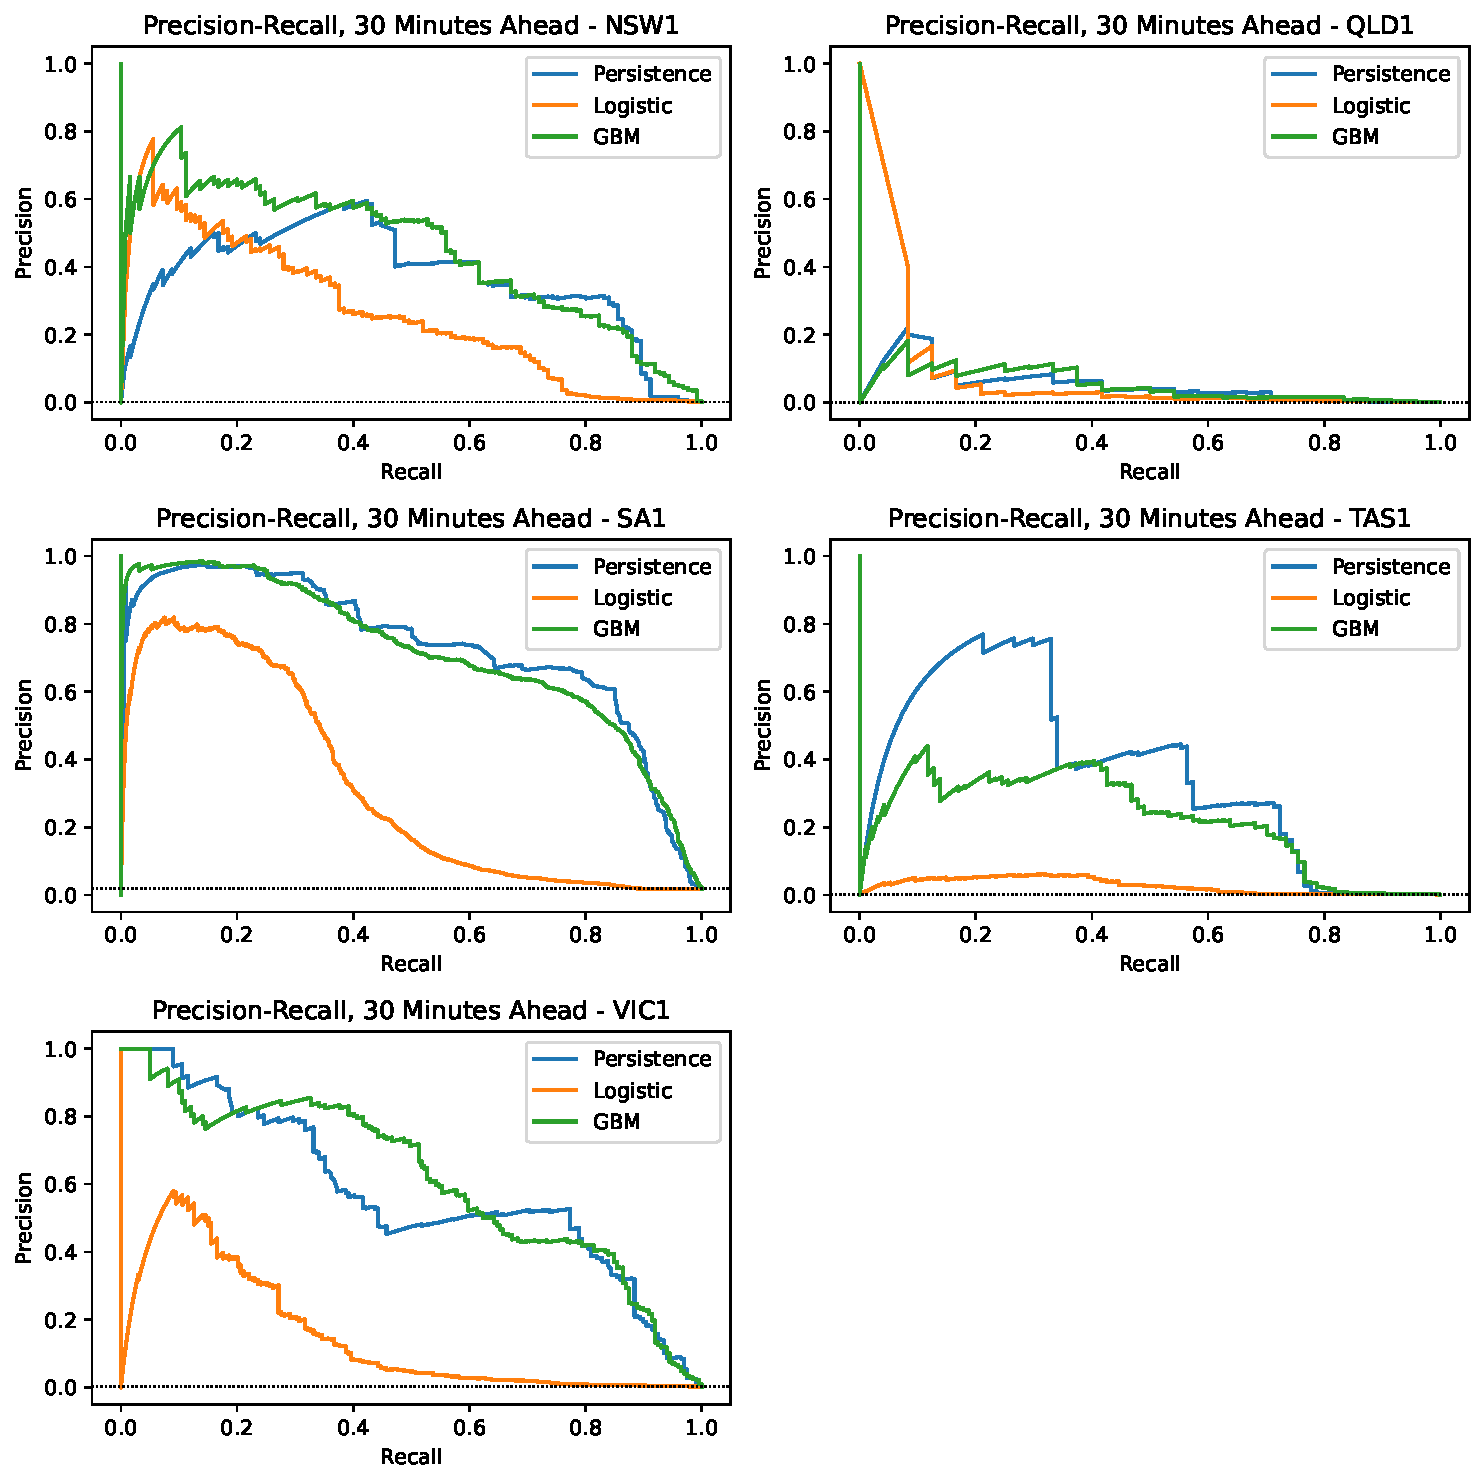
\includegraphics[width=0.8\textwidth]{pr_curves.pdf}
\caption{Precision--recall curves 30 minutes ahead. The dotted line is the base rate.}\label{fig:pr}
\end{figure}

\textbf{Calibration.} The reliability diagram (Figure \ref{fig:reliability}) bins forecasts on a log scale and plots the observed frequency with a Wilson 95\% interval \cite{wilson1927}. The GBM's probabilities lie close to the diagonal in every region, slightly
under-forecasting in the middle of the range. Logistic regression is badly calibrated at the extremes, over-forecasting its
highest probabilities in TAS1 and under-forecasting its lowest in SA1.

\begin{figure}[!htbp]\centering
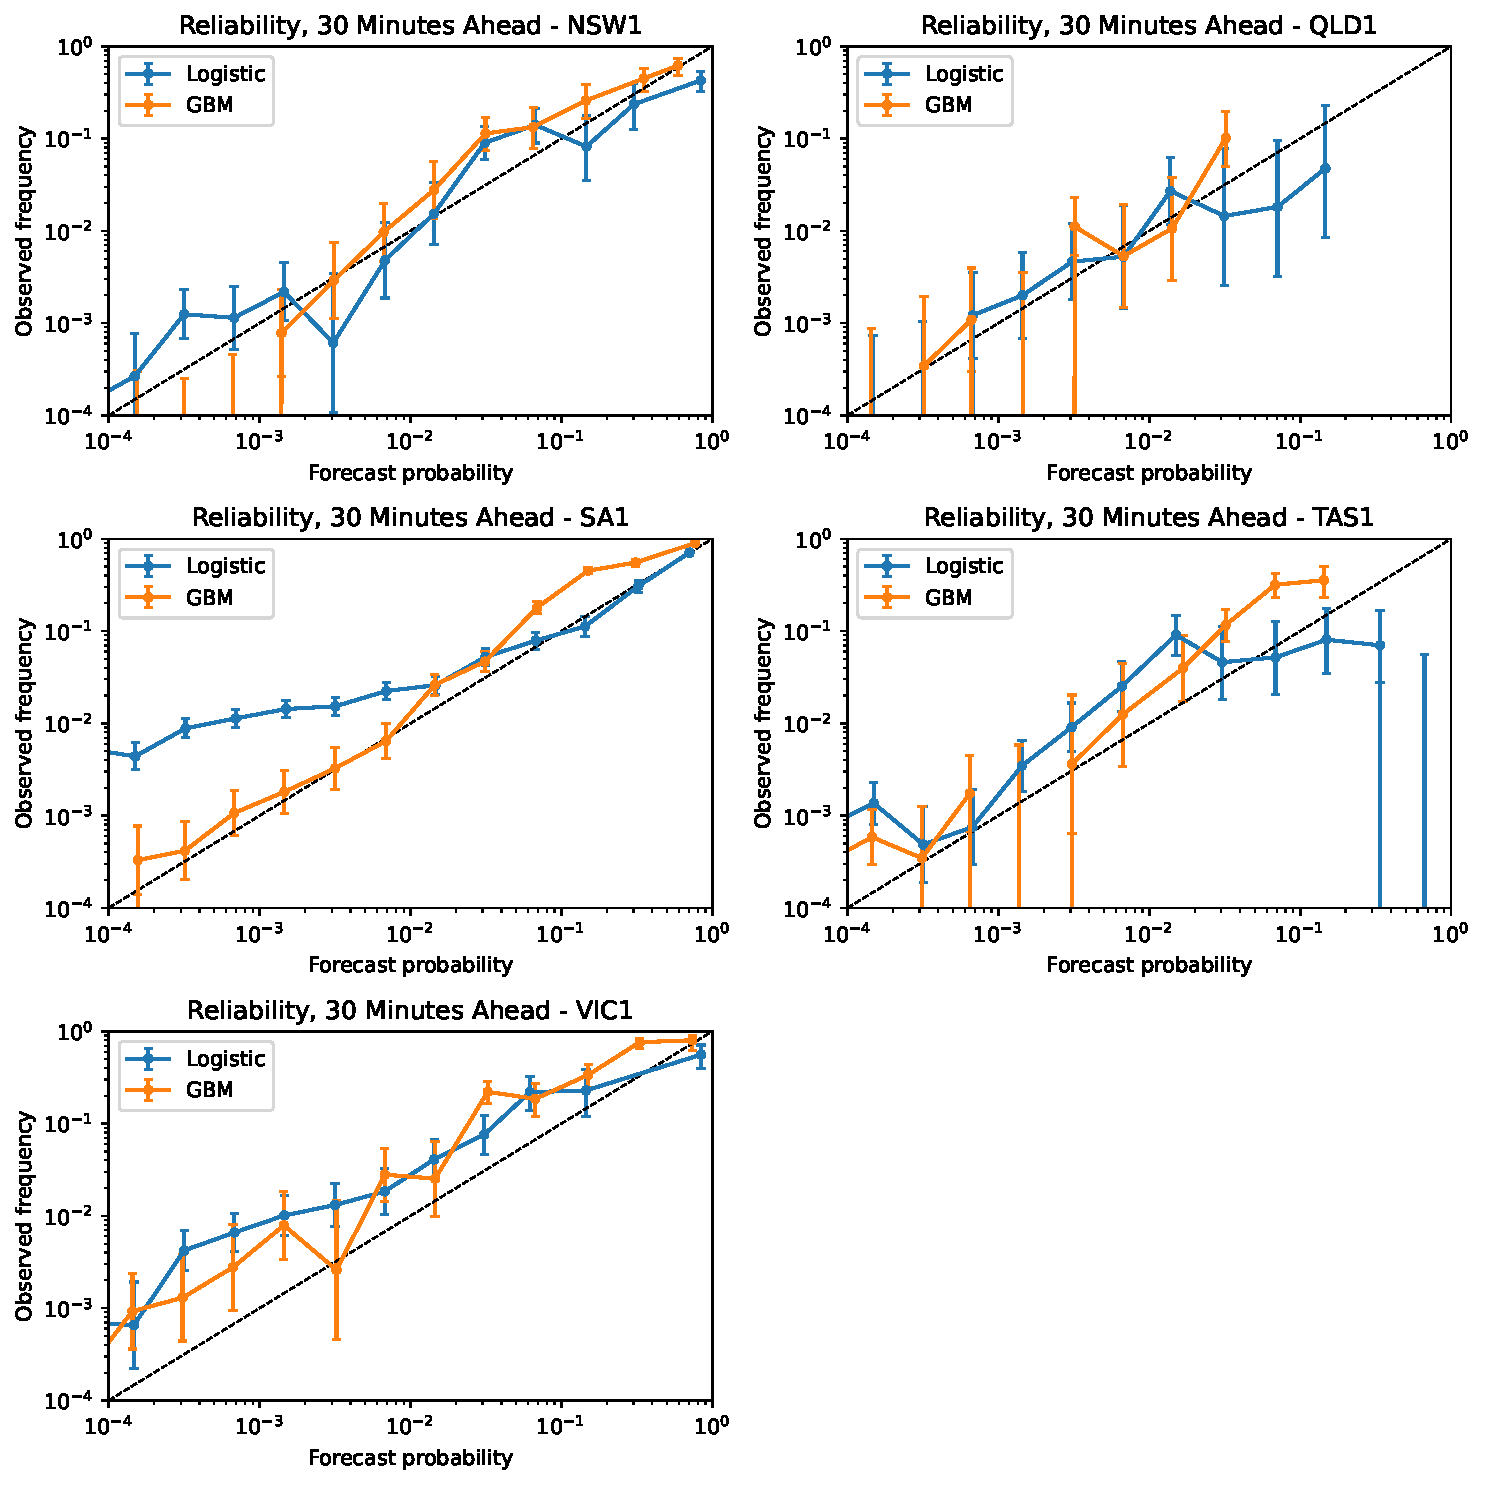
\includegraphics[width=0.8\textwidth]{reliability.pdf}
\caption{Reliability diagrams 30 minutes ahead, with Wilson 95\% intervals.}\label{fig:reliability}
\end{figure}

\textbf{What does the GBM use?} Grouped permutation importance shuffles all columns of a feature group together and measures the drop in AP (Table \ref{tab:importance}). The price itself does almost all the work. Supply in
NSW1 (0.07), and to a lesser extent network in NSW1 and constraints in TAS1 (both 0.02), are the only other groups that clearly
help. The excitation features add almost nothing, even though the Hawkes fit says spikes trigger spikes: the price history
already carries that information.

\begin{table}[!htbp]\centering\small
\caption{Grouped permutation importance of the GBM, 30 minutes ahead: drop in AP when the group is shuffled, weighted by spikes per test month.}\label{tab:importance}
\begin{tabular}{lrrrrr}
\toprule
region & NSW1 & QLD1 & SA1 & TAS1 & VIC1 \\
group & & & & & \\
\midrule
own\_price & 0.495 & 0.087 & 0.678 & 0.438 & 0.645 \\
constraints & 0.005 & -0.001 & -0.001 & 0.035 & 0.000 \\
calendar & -0.003 & -0.008 & 0.000 & 0.000 & 0.034 \\
supply & 0.073 & -0.019 & 0.011 & -0.048 & 0.006 \\
excitation & 0.000 & -0.001 & 0.001 & 0.004 & 0.000 \\
fcas & -0.005 & 0.004 & -0.000 & -0.032 & 0.003 \\
neighbours & 0.001 & -0.044 & 0.007 & -0.002 & 0.004 \\
network & 0.005 & 0.011 & -0.009 & -0.066 & 0.023 \\
\bottomrule
\end{tabular}
\end{table}

\textbf{Why anchor the GBM?} Switching off each design choice (Table \ref{tab:ablation}) shows the anchor matters most. Without it
AP falls in every region, badly in TAS1 (0.27 to 0.12) and VIC1 (0.59 to 0.38), and without both choices it is worse again
everywhere. Dropping only the monotone constraints hurts in NSW1 (0.52 to 0.42), barely matters in SA1 and VIC1, and helps
slightly in TAS1. We also checked the number of trees: the test loss bottoms out between 25 and 300 trees depending on the region,
so the fixed 200 trees slightly overfit in SA1, TAS1 and VIC1, but with this little spike data there is no reliable way to pick
the number per region in advance.

\begin{table}[!htbp]\centering\small
\caption{GBM ablation: AP 30 minutes ahead with each design choice switched off.}\label{tab:ablation}
\begin{tabular}{lrrrrrrrr}
\toprule
model & \multicolumn{2}{r}{GBM} & \multicolumn{2}{r}{GBM no anchor} & \multicolumn{2}{r}{GBM no monotone} & \multicolumn{2}{r}{GBM neither} \\
 & AP & AP\_onset & AP & AP\_onset & AP & AP\_onset & AP & AP\_onset \\
\midrule
NSW1 & 0.452 & 0.193 & 0.451 & 0.169 & 0.453 & 0.165 & 0.408 & 0.149 \\
QLD1 & 0.057 & 0.036 & 0.089 & 0.062 & 0.040 & 0.026 & 0.035 & 0.027 \\
SA1 & 0.717 & 0.176 & 0.662 & 0.155 & 0.713 & 0.174 & 0.629 & 0.144 \\
TAS1 & 0.225 & 0.029 & 0.116 & 0.020 & 0.252 & 0.027 & 0.074 & 0.013 \\
VIC1 & 0.615 & 0.128 & 0.428 & 0.088 & 0.594 & 0.145 & 0.353 & 0.076 \\
\bottomrule
\end{tabular}
\end{table}
